\chapter{Technical report}
%\chapter{Application à la Transmission d’un fichier quelconque (*.mpeg, *.mp3, *.txt, *.doc, *.pdf, etc)}

%\minitoc


\section{Explanations on Eigenface prototype}
In this section, we will explain the implementation of  eigenfaces  method  with the differents expressions  
\subsection{Algorithm}
Using mostly PCA (principal components Analysis),eigenfaces method is based on the calculation of eigenvectors and eigenvalues.
The algorithm consists of two steps: The learning phase and the identification phase

\subsubsection{learning phase}
 The learning phase can be divided in several steps:
 \begin{itemize}
 \item Step 1 : It is necessary to have an image database consisting of M images. In our case we used the basis of ATT pictures composed of 400 images. The database consists of 40 subjects and each subject has 10 images. All these images are the basis for learning.Each image is a matrix.
 \item Step 2 :Each image matrix is converted into vector










\parbox{0.60\linewidth}{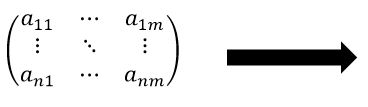
\includegraphics[scale=0.75]{matrice2vector}%[height=70mm,width=70mm]
}
\parbox{0.15\linewidth}{


%\begin{figure}[bth]%[!ht]
%\begin{center}
%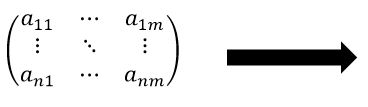
\includegraphics[scale=0.75]{matrice2vector}%[height=70mm,width=70mm]
%\caption{\textbf{conversion matrix to vector}}%
%%\url {http://www.google.fr/}
%\label{matrice2vector}%
%\end {center}
%\end{figure} 
\begin{displaymath} A=\left[\begin{array}{ccc}
a_{11} \\
\vdots \\
a_{nm} 
\end{array}\right] \end{displaymath}
}



\item Step 3 : all M image vectors are then combined into a single  matrix $\Gamma$. Note that each column of the matrix represents an image $\Gamma_{i}$.
\begin{figure}[bth]%[!ht]
\begin{center}
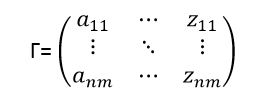
\includegraphics[scale=0.75]{grandematrice}%[height=70mm,width=70mm]
\caption{\textbf{matrix of images database}}%
%\url {http://www.google.fr/}
\label{grandematrice}%
\end {center}
\end{figure} 
\\a:the subject 1 and z the subject n
\newpage
\item Step 4 : Calculate the average $\Psi$ of all images
\begin{figure}[bth]%[!ht]
\begin{center}
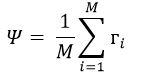
\includegraphics[scale=0.75]{moyenne}%[height=70mm,width=70mm]
%\caption{\textbf{average image}}%
%\url {http://www.google.fr/}
\label{moyenne}%
\end {center}
\end{figure} 
\item Step 5 :  substract the average image  from each image
\begin{figure}[bth]%[!ht]
\begin{center}
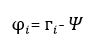
\includegraphics[scale=0.75]{centrage}%[height=70mm,width=70mm]
%\caption{\textbf{average image}}%
%\url {http://www.google.fr/}
\label{centrage}%
\end {center}
\end{figure}
\item Step 6 : calculate the covariance matrix S
\begin{figure}[bth]%[!ht]
\begin{center}
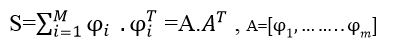
\includegraphics[scale=0.75]{cov_matrix}%[height=70mm,width=70mm]
%\caption{\textbf{average image}}%
%\url {http://www.google.fr/}
\label{centrage}%
\end {center}
\end{figure}
\item Step 7 : After the covariance matrix ,eigenvalues and eigenvectors are computed.
Eigenvectors are then sorted by decreasing order.
%\begin{center}
%	\begin{tabular}{ll}
%	&\begin{math}
%		\sin \theta_{c} = n_{1}*\sin i_{c}\par \vspace{0.25cm}
%	\end{math}
%	\\

%{\color{red} \textbf{Formule de Snell-Descartes} :} & $n_{0}*\sin \theta_{c} = n_{1}*\sin i_{c}$ \\
%&  avec $n_{0} = 1$ (\emph{air})
%\end{tabular}
%\end{center}

\begin{math}
   S * e_{i} =  \lambda_{i} * e_{i}
\end{math}


Formulas :
 $ \left\{\begin{array}{rl}
e_{i}= A * v_{i} & \mbox{eigenvectors } \\
\lambda_{i} = \mu_{i} & \mbox{eigenvalues
}\end{array}\right.$



  \end{itemize}
  
\subsubsection{identification phase}  
The identification phase consists of two steps and   will help to  recognize an input image in the image database.
 \begin{itemize}
 \item Step 1 : compute projection vectors
 
\begin{math}
   w_{k} = e^t_{k} * (\lambda_{i} -\psi)
\end{math} 
 
 
 

\paragraph{}
The projection vectors are called "weight vectors " and form a single matrix which will help for  compute  Euclidean distance. It also will help to find the class for an  input image.
\item Step 2 : compute the Euclidian distance
 
 \end {itemize}




 



%\begin{figure}[bth]%[!ht]
%\begin{center}
%\includegraphics[scale=0.75]{nom_image}%[height=70mm,width=70mm]
%\caption{\textbf{Titre image}}%
%\url {http://www.google.fr/}
%\label{label_image}%
%\end {center}
%\end{figure}

\subsection{Functions programmed}
\section{Explanations on Fisherface prototype}
\subsection{Alorithm}
\subsection{Functions programmed}